\subsection{Room allocation: exact reference and predicted search quality}
\label{sec:room-results}

The room fixture has seven predicted durations of 30--90 minutes in ten-minute
increments, two rooms and $2^7=128$ allocations. Enumeration gives $U=0$,
$O=165$ and $C_{\mathrm{room}}=0.313688$. Table~\ref{tab:room-exact} shows
that all five searches reach this optimum at every tested seed; the greedy
baseline has an absolute cost gap of 0.80038. This is a predicted allocation certificate only: without closure, hidden
durations leave mean completions at 5.67--6 of seven cases across methods.

\begin{table}[H]
\centering\small
\caption{Small room-allocation reference: absolute initial predicted-cost gaps, exact hits and mean initial solve time. Three seeds on one fixed seven-case fixture; baseline repeats are identical.}
\label{tab:room-exact}
\begin{tabular}{@{}lrrrr@{}}
\toprule
Method & Mean gap & Worst gap & Exact hits & Time (s) \\
\midrule
Baseline & 0.80038 & 0.80038 & 0/3 & 0.000 \\
SA & 0.00000 & 0.00000 & 3/3 & 0.523 \\
Tabu & 0.00000 & 0.00000 & 3/3 & 0.521 \\
GA & 0.00000 & 0.00000 & 3/3 & 0.523 \\
Hybrid & 0.00000 & 0.00000 & 3/3 & 0.538 \\
ACO & 0.00000 & 0.00000 & 3/3 & 0.574 \\
\bottomrule
\end{tabular}
\end{table}


Table~\ref{tab:room-initial} separates predicted initial quality from execution.
At 100 cases, SA, tabu and the hybrid reduce mean predicted overtime from
668.0 minutes for the baseline to 602.0. At 300 cases, tabu and the hybrid
reach 1905.5 versus 2195.0 for the baseline; SA reaches 1908.0. All retain
zero predicted unstarted cases. GA retains the incumbent at both sizes;
ACO improves it at 100 cases but not at 300. These rankings are specific to the tested budget.

\begin{table}[H]
\centering\small
\caption{Generated workloads: initial predicted unstarted count U, overtime OT and end-to-end solve time, averaged over six plans per method and size. These predicted quantities are distinct from execution outcomes. The 300-case campaign used four concurrent batches.}
\label{tab:room-initial}
\begin{tabular}{@{}rlrrr@{}}
\toprule
Cases & Method & Predicted U & Predicted OT & Time (s) \\
\midrule
100 & Baseline & 0.00 & 668.0 & 0.002 \\
100 & SA & 0.00 & 602.0 & 0.696 \\
100 & Tabu & 0.00 & 602.0 & 0.679 \\
100 & GA & 0.00 & 668.0 & 0.697 \\
100 & Hybrid & 0.00 & 602.0 & 0.682 \\
100 & ACO & 0.00 & 616.2 & 1.366 \\
300 & Baseline & 0.00 & 2195.0 & 0.009 \\
300 & SA & 0.00 & 1908.0 & 1.098 \\
300 & Tabu & 0.00 & 1905.5 & 1.107 \\
300 & GA & 0.00 & 2195.0 & 1.128 \\
300 & Hybrid & 0.00 & 1905.5 & 1.089 \\
300 & ACO & 0.00 & 2195.0 & 3.707 \\
\bottomrule
\end{tabular}
\end{table}


The mean initial time is approximately 0.68--0.70 seconds for the four
non-ACO searches at 100 cases, compared with 1.37 seconds for ACO. At
300 cases, corresponding means are approximately 1.09--1.13 and 3.71 seconds.
Baseline timing excludes a search worker. Per-candidate work differs, and
concurrent 300-case execution limits cross-size timing interpretation. Larger
room instances have no certified optimum or optimality gap.

\subsection{Static and reactive execution under room closure}

Historical outcomes vary by day (Table~\ref{tab:room-historical}). All methods
complete nine cases on 3 January under both policies, but reactive overtime
is higher. On 2 February, tabu and the hybrid move from 12.00 completed cases
and 158.7 overtime minutes under static execution to 11.33 and 108.0 under
reactive execution. Lower overtime here accompanies fewer completed cases.
On 20 October, all methods complete 16 of 25 cases under both policies, while
reactive overtime falls from 110 minutes to about 73.7--82.7. Day-level comparisons therefore matter.

\begin{table}[H]
\centering\small
\caption{Historical closure scenario: mean completed cases and realised overtime over three solver seeds per day. S = static; R = reactive. Each pair shares its initial plan. Overtime includes turnover and sums minutes over rooms.}
\label{tab:room-historical}
\begin{tabular}{@{}llrrrr@{}}
\toprule
Date & Method & Done S & Done R & OT S & OT R \\
\midrule
2022-01-03 & Baseline & 9.00 & 9.00 & 64.0 & 92.0 \\
2022-01-03 & SA & 9.00 & 9.00 & 7.3 & 44.7 \\
2022-01-03 & Tabu & 9.00 & 9.00 & 15.7 & 57.3 \\
2022-01-03 & GA & 9.00 & 9.00 & 61.0 & 95.0 \\
2022-01-03 & Hybrid & 9.00 & 9.00 & 15.7 & 57.3 \\
2022-01-03 & ACO & 9.00 & 9.00 & 10.3 & 41.0 \\
2022-02-02 & Baseline & 11.00 & 11.00 & 59.0 & 113.0 \\
2022-02-02 & SA & 11.67 & 11.33 & 135.3 & 109.3 \\
2022-02-02 & Tabu & 12.00 & 11.33 & 158.7 & 108.0 \\
2022-02-02 & GA & 11.67 & 11.00 & 115.0 & 68.0 \\
2022-02-02 & Hybrid & 12.00 & 11.33 & 158.7 & 108.0 \\
2022-02-02 & ACO & 11.67 & 11.33 & 154.7 & 121.3 \\
2022-10-20 & Baseline & 16.00 & 16.00 & 110.0 & 77.0 \\
2022-10-20 & SA & 16.00 & 16.00 & 110.0 & 74.0 \\
2022-10-20 & Tabu & 16.00 & 16.00 & 110.0 & 75.7 \\
2022-10-20 & GA & 16.00 & 16.00 & 110.0 & 73.7 \\
2022-10-20 & Hybrid & 16.00 & 16.00 & 110.0 & 75.7 \\
2022-10-20 & ACO & 16.00 & 16.00 & 110.0 & 82.7 \\
\bottomrule
\end{tabular}
\end{table}


The generated closure workloads also show mixed effects
(Table~\ref{tab:room-generated}). At 300 cases, baseline replanning raises
mean completions from 287.5 to 289.5 and overtime from 2838.0 to 3319.5
room-minutes. Tabu and the hybrid begin at 289.0 completions under static
execution and fall to 287.33 and 287.50 respectively when reactive. These
policy differences are conditional on each method's shared initial plan;
they do not compare methods from a common initial allocation.

\begin{table}[H]
\centering\small
\caption{Generated closure scenario: means over two sampled workloads and three solver seeds (six runs per cell). Resources are 14/15 rooms for 100 cases and 44/45 for 300 cases. OT is realised overtime including turnover, in room-minutes.}
\label{tab:room-generated}
\begin{tabular}{@{}rlrrrr@{}}
\toprule
Cases & Method & Done S & Done R & OT S & OT R \\
\midrule
100 & Baseline & 97.00 & 97.00 & 933.5 & 1022.0 \\
100 & SA & 96.67 & 96.17 & 952.5 & 958.5 \\
100 & Tabu & 96.50 & 95.67 & 876.0 & 856.0 \\
100 & GA & 97.00 & 96.33 & 933.5 & 971.7 \\
100 & Hybrid & 96.50 & 96.17 & 876.0 & 932.8 \\
100 & ACO & 96.33 & 96.00 & 902.5 & 976.0 \\
300 & Baseline & 287.50 & 289.50 & 2838.0 & 3319.5 \\
300 & SA & 287.33 & 286.33 & 2923.0 & 3028.5 \\
300 & Tabu & 289.00 & 287.33 & 3021.5 & 3140.5 \\
300 & GA & 287.50 & 286.00 & 2838.0 & 2974.5 \\
300 & Hybrid & 289.00 & 287.50 & 3021.5 & 3165.5 \\
300 & ACO & 287.50 & 285.17 & 2838.0 & 3000.5 \\
\bottomrule
\end{tabular}
\end{table}


Across all 144 closure pairs, reactive execution completes more cases in 16,
the same number in 83 and fewer in 45. Overtime falls in 64, ties in seven
and rises in 73. The counts include deterministic baseline repeats and are descriptive.
All no-closure static/reactive pairs have identical completion, overtime,
occupancy and total delay, as expected when no replanning trigger occurs.

\begin{figure}[H]
\centering
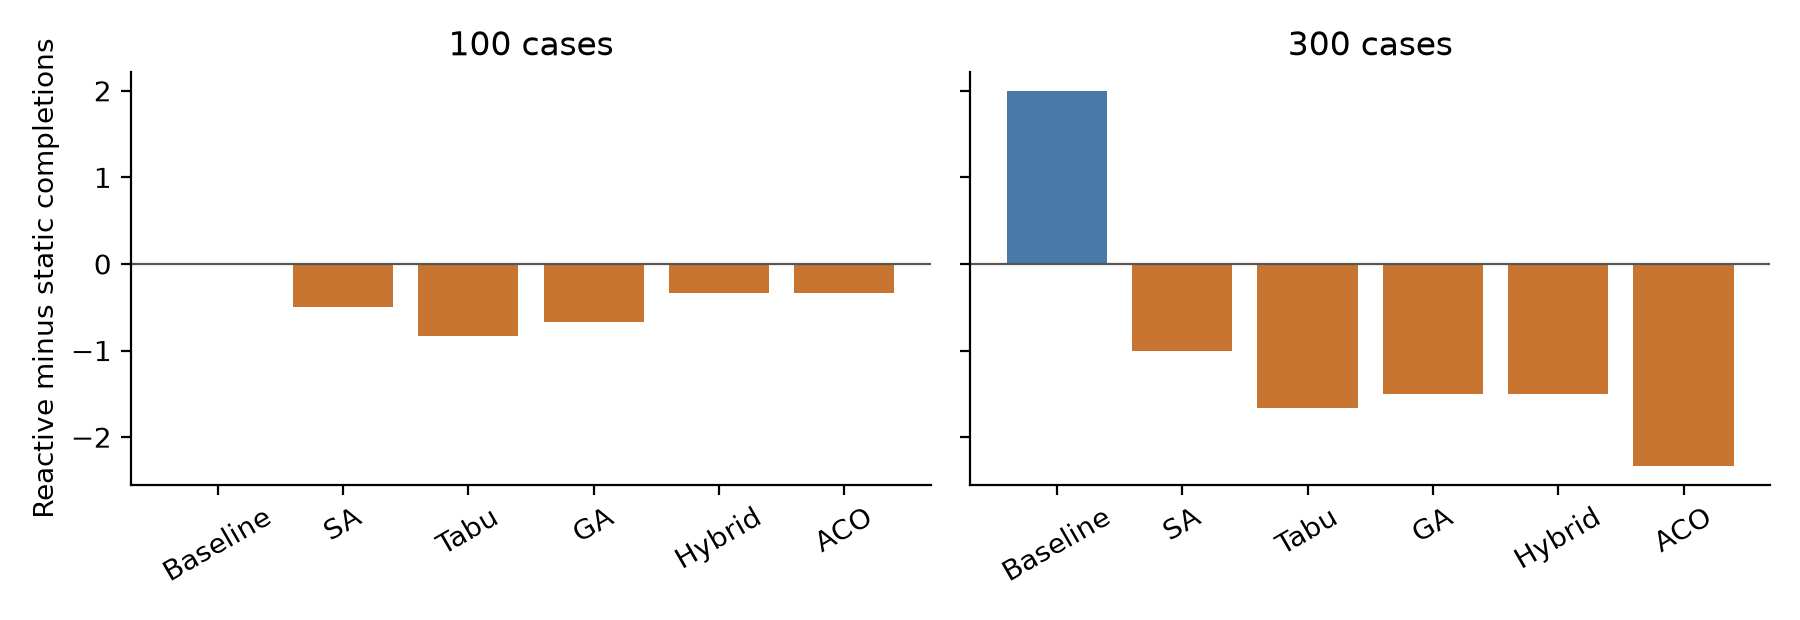
\includegraphics[width=0.95\linewidth]{figures/room-policy-differences.png}
\caption{Mean paired completion differences under closure in the primary
room campaign. Each bar averages two generated workloads and three solver
seeds; positive values favour reactive execution. No confidence intervals
or statistical superiority are claimed. Read alongside overtime in
Table~\ref{tab:room-generated}.}
\label{fig:room-policy}
\end{figure}

\subsection{Perfect duration information: a separate execution comparison}
\label{sec:duration-results}

Table~\ref{tab:room-duration} uses the separate median/oracle campaign,
restricting the displayed comparison to no-closure static execution so
neither disruption nor reactive replanning changes between modes. At 300
cases, oracle estimates allow all six methods to complete 300 cases on average,
compared with 287.5--289.17 under median estimates. Oracle overtime is
3590.5--3678.0 room-minutes, compared with 2779.0--2965.0: additional throughput
comes with more post-closing occupancy, consistent with the objective's
priority for case starts.

\begin{table}[H]
\centering\small
\caption{Separate duration-information campaign: no-closure static execution. M = historical-median estimates; O = oracle durations. Means use two workloads and three solver seeds. Resources and hidden outcomes are held fixed across modes; initial plans are recomputed. OT includes turnover.}
\label{tab:room-duration}
\begin{tabular}{@{}rlrrrr@{}}
\toprule
Cases & Method & Done M & Done O & OT M & OT O \\
\midrule
100 & Baseline & 97.50 & 99.50 & 922.0 & 886.0 \\
100 & SA & 97.17 & 100.00 & 942.7 & 908.5 \\
100 & Tabu & 97.17 & 100.00 & 874.7 & 908.5 \\
100 & GA & 97.50 & 99.50 & 922.0 & 883.3 \\
100 & Hybrid & 97.17 & 100.00 & 874.7 & 908.5 \\
100 & ACO & 97.17 & 100.00 & 908.5 & 927.5 \\
300 & Baseline & 287.50 & 300.00 & 2779.0 & 3678.0 \\
300 & SA & 288.00 & 300.00 & 2949.7 & 3590.5 \\
300 & Tabu & 289.17 & 300.00 & 2965.0 & 3590.5 \\
300 & GA & 287.50 & 300.00 & 2779.0 & 3678.0 \\
300 & Hybrid & 289.17 & 300.00 & 2965.0 & 3590.5 \\
300 & ACO & 287.50 & 300.00 & 2779.0 & 3678.0 \\
\bottomrule
\end{tabular}
\end{table}


At 100 cases, the four non-GA searches complete all 100 cases under oracle
estimates, whereas baseline and GA complete 99.5 on average. In the small
fixture, each metaheuristic completes all seven cases with 240 overtime
minutes under oracle information; the baseline still completes six with
105 minutes. Perfect information therefore does not compensate for every
search or representation restriction, nor does it necessarily lower overtime.
Duration substitution also changes ordering and search landscape. Learned
models require their own held-out end-to-end comparison; oracle gains do
not estimate their operational benefit.
